\documentclass[11pt]{article}
\usepackage[T1]{fontenc}
\usepackage[utf8]{inputenc}
\usepackage{amsmath,amssymb,booktabs,graphicx}
\usepackage[margin=0.9in]{geometry}
\usepackage[colorlinks=true,urlcolor=blue,citecolor=blue,linkcolor=blue]{hyperref}
\setlength{\parskip}{0.45em}
\setlength{\parindent}{0pt}
\title{Radion stability and brane couplings in a reflection-symmetric five-dimensional interval}
\author{Hicham Boufourou}
\date{Research draft -- 5 September 2026}
\begin{document}
\maketitle
\begin{abstract}
We study a five-dimensional physical interval with a canonical bulk scalar, a convex quadratic bulk potential and linear boundary potentials. The reconstructed Minkowski backgrounds are reflection symmetric, have an odd scalar profile, and possess an interior maximum of the warp factor. A regular scalar variable gives a generalized Sturm--Liouville problem whose positive bulk and boundary quadratic forms establish strictly positive scalar squared masses at every smooth branch point with nonzero scalar gradient. We derive canonical same-brane couplings and closed weak-backreaction coefficients for x = \(\mu\)L: \(\kappa\)(x) = 4x tanh(x/2)sech\({}^2\)(x/2) for m\({}_r\)\({}^2\)L\({}^2\)/\(\epsilon\)\({}^2\), and c\(\alpha\)(x) = sech\({}^2\)(x/2)[1 + tanh\({}^2\)(x/2) + 2tanh(x/2)/x] for 3\(\alpha\)\({}_r\) - 1 at order \(\epsilon\)\({}^2\). The coupling correction is positive for each fixed x > 0. A leading effective-potential calculation checks the mass, and finite-backreaction numerical benchmarks illustrate the joint evolution of masses and residues. The analysis applies established perturbation methods to a specified effective family. It neither selects an absolute compactification length nor claims experimental viability or a derivation from DDF geometry.
\end{abstract}
\section*{1. Introduction and scope}
A compact fifth dimension contains a scalar gravitational degree of freedom associated with its proper length. Stabilizing this degree of freedom and determining its coupling to matter are related but distinct tasks. A massive radion need not have a negligible coupling, and an assumed compactification length does not become a prediction merely because a stable background can be constructed. Bulk-scalar stabilization and fully backreacted scalar--gravity backgrounds have a substantial history [1,2]. The present work studies one explicitly specified effective model within that framework.

The model is a physical interval supported by a canonical scalar with a convex quadratic bulk potential and linear boundary potentials. Its background is invariant under reflection about the midpoint combined with reversal of the scalar. The warp factor has a maximum in the interior and takes the same value on the two boundaries. Scalar fluctuation equations, exact canonical normalization, and brane couplings have already been developed for broad classes of backgrounds [3,4]. We apply these established methods to the present family and give the convention choices, endpoint terms, perturbative coefficients, and numerical checks needed to make the calculation reproducible.

The main analytical results are a positive generalized Sturm--Liouville formulation valid through the interior zero of the warp derivative, and closed weak-backreaction expressions for the light-mode mass and brane coupling as functions of x = \(\mu\)L. The latter show that, for fixed x > 0 and sufficiently weak stabilization, the radion coupling increases above its flat value. This is a model-dependent statement, not a universal relation between radion mass and coupling. We also report finite-backreaction benchmarks and distinguish the single-radion contribution from the complete scalar and tensor exchange signal.

This study was motivated by efforts to isolate a consistent effective sector of the DDF research project. No derivation of the action from a Calabi--Yau compactification or other proposed DDF geometry is assumed here. The proper interval length remains an input unless the dimensionful stabilizer parameters are independently specified. The paper therefore makes no claim of detecting an extra dimension, predicting a micrometric radius, explaining the observed vacuum energy, or satisfying short-distance gravity constraints. Its intended contribution is a reproducible analytical and numerical model study; priority for the specific closed coefficients remains subject to further literature review.

\section*{2. Physical-interval action and reconstructed backgrounds}
We use signature (-++++) and integrate once over a physical interval 0 \(\leq\) y \(\leq\) L. The gravitational coefficient is M\({}_5\)\({}^3\)/2; changing it while keeping the equations below would change the theory. The Gibbons--Hawking--York boundary term and outward-normal orientations \(\eta\)\({}_0\) = -1 and \(\eta\)L = +1 are included. The action is

\begin{equation}
S=\int_0^L dy\int d^4x\sqrt{-g}\left[\frac{M_5^3}{2}\mathcal{R}-\frac{1}{2}(\partial\sigma)^2-V(\sigma)\right]\tag{1a}
\end{equation}
\begin{equation}
\quad+M_5^3\int_{\partial M}d^4x\sqrt{-\gamma}\,K-\sum_i\int_i d^4x\sqrt{-\gamma}\,U_i(\sigma)+S_m[\gamma_0]\tag{1b}
\end{equation}
\begin{equation}
V(\sigma)=\Lambda_5+\frac{1}{2}\mu^2\sigma^2,\qquad U_i(\sigma)=T_i+J_i\sigma.\tag{2}
\end{equation}
Matter is minimally coupled to the induced metric of the left boundary. There is no independent direct coupling of matter to the stabilizer, no brane kinetic term for the scalar, and no induced Einstein term. No additional bulk scalar is included. These restrictions are part of the model, since each omitted interaction can alter the normal-mode problem or its observable residues.

For Minkowski slices and a proper-distance coordinate, the background metric and equations are

\begin{equation}
ds^2=e^{2A(y)}\eta_{\mu\nu}dx^\mu dx^\nu+dy^2,\qquad A^{\prime\prime}=-\frac{\sigma^{\prime 2}}{3M_5^3},\tag{3}
\end{equation}
\begin{equation}
6M_5^3 A^{\prime 2}=\frac{\sigma^{\prime 2}}{2}-\Lambda_5-\frac{\mu^2\sigma^2}{2},\qquad \sigma^{\prime\prime}=\mu^2\sigma-4A^\prime\sigma^\prime.\tag{4}
\end{equation}
\begin{equation}
U_i=3\eta_i M_5^3 A_i^\prime,\qquad J_i=-\eta_i\sigma_i^\prime.\tag{5}
\end{equation}
Equation (5) is the junction convention appropriate to this single physical interval. The calculation does not multiply the bulk action by a second orbifold copy. All Planck masses, scalar norms, and source couplings below use the same interval convention.

We choose \(\mu\) > 0 and a regular reflection-symmetric solution with \(\sigma\)(L/2) = A\({}^\prime\)(L/2) = 0 and \(\sigma\)\({}^\prime\)(L/2) > 0. The scalar is odd about the midpoint; A and \(\sigma\)\({}^\prime\) are even. Fixing the endpoint derivative q = \(\sigma\)\({}^\prime\)(0) = \(\sigma\)\({}^\prime\)(L) > 0 implies J\({}_0\) = q and JL = -q. An additive shift sets A(0) = A(L) = 0, so masses are measured in the physical coordinates of either brane. We define

\begin{equation}
x=\mu L,\qquad \epsilon=\frac{qL}{\sqrt{12M_5^3}}.\tag{6}
\end{equation}
Numerically, L = M\({}_5\)\({}^3\) = 1 is a choice of units. A shot from the center adjusts the central scalar derivative to achieve the chosen q. The constraint then fixes \(\Lambda\)\({}_5\) = \(\sigma\)\({}^\prime\)(L/2)\({}^2\)/2 > 0. Finally, the tensions are reconstructed as Ti = 3\(\eta\)i M\({}_5\)\({}^3\)A\({}^\prime\)i - Ji\(\sigma\)i. Each background is a solution of the action with these reconstructed constants. Comparing different \(\epsilon\), or different x, generally compares different actions. It does not follow the radius at fixed values of every coupling.

There are two immediate qualifications. First, Minkowski slicing requires tuning the vacuum energy; it is not a calculation of the observed cosmological constant. Second, concavity of A makes the background localized energies Ui negative at both endpoints on this branch. The bulk scalar obeys the usual null-energy condition, but positive endpoint energy is not an assumption of this model. The fixed-boundary effective description and its linear stability do not provide a microscopic realization of these boundary sources.

\section*{3. Regular scalar perturbations and boundary conditions}
In a gauge with the boundaries at fixed coordinates, write the scalar perturbations using a four-dimensional mode \(\chi\). The exponential metric parametrization is convenient for the quadratic kinetic calculation; the background and junction equations are assumed to hold.

\begin{equation}
ds^2=e^{2A+2F}\eta_{\mu\nu}dx^\mu dx^\nu+e^{-4F}dy^2,\qquad F=f(y)\chi(x),\tag{7}
\end{equation}
\begin{equation}
\delta\sigma=s(y)\chi(x),\qquad (\Box_4-m^2)\chi=0.\tag{8}
\end{equation}
The mixed Einstein equation gives the constraint below. The remaining scalar equation can be written in the familiar proper-coordinate form [3], with signs adjusted to the metric convention in (7):

\begin{equation}
3M_5^3(f^\prime+2A^\prime f)+\sigma^\prime s=0,\qquad W=\frac{\sigma^{\prime\prime}}{\sigma^\prime},\tag{9}
\end{equation}
\begin{equation}
f^{\prime\prime}+(2A^\prime-2W)f^\prime+(4A^{\prime\prime}-4A^\prime W+m^2e^{-2A})f=0.\tag{10}
\end{equation}
This representation requires a nonzero scalar gradient, but never divides by A\({}^\prime\). It is therefore regular at the midpoint, where the warp derivative vanishes. Regularity of the chosen branch implies \(\sigma\)\({}^\prime\) > 0 throughout the interval: on its right half, \(\sigma\) > 0 and A\({}^\prime\) < 0, so (4) drives \(\sigma\)\({}^\prime\) upward rather than toward zero. Reflection covers the other half.

For a linear physical boundary potential, U\({}^{\prime\prime}\)i = 0. Perturbing the normal scalar junction gives s\({}^\prime\) + 2\(\sigma\)\({}^\prime\)f = 0 at both endpoints. Let B = f\({}^\prime\) + 2A\({}^\prime\)f. Equation (10) implies B\({}^\prime\) = 2WB - 2A\({}^{\prime\prime}\)f - m\({}^2\)e\({}^-\)\({}^2\)\({}^A\)f. Using (9) and the background equation then gives

\begin{equation}
W_i(f_i^\prime+2A_i^\prime f_i)-m^2e^{-2A_i}f_i=0.\tag{11}
\end{equation}
No division by m\({}^2\) was used in this derivation. A putative propagating scalar zero mode can thus be tested in the same regular problem when q > 0. A mode with null four-momentum still obeys the momentum constraint; a strictly constant deformation of the action parameters is not a propagating mode of a fixed action. The case q = 0 is separately degenerate because (9) cannot then be solved for s using \(\sigma\)\({}^\prime\).

\section*{4. Linear spectral stability without dividing by the warp derivative}
Stability criteria depend on the boundary conditions, and a numerical list of positive roots is not a proof that negative roots are absent. We give the positive quadratic form directly. This is a specialization of established scalar--gravity Sturm--Liouville methods [5,6], not a new general stability criterion.

\begin{equation}
g=e^{2A}f,\quad p=\frac{e^{-2A}}{\sigma^{\prime 2}},\quad w=\frac{e^{-4A}}{\sigma^{\prime 2}},\quad Q=-2A^{\prime\prime}p=\frac{2e^{-2A}}{3M_5^3}.\tag{12}
\end{equation}
\begin{equation}
-(pg^\prime)^\prime+Qg=m^2wg,\qquad g_i^\prime=\frac{m^2e^{-2A_i}}{W_i}g_i.\tag{13}
\end{equation}
For every smooth finite background of the specified branch, p, w and Q are positive. Moreover, W = \(\mu\)\({}^2\)\(\sigma\)/\(\sigma\)\({}^\prime\) - 4A\({}^\prime\) is positive on the right half away from the midpoint. Consequently WL > 0 and W\({}_0\) < 0. Multiplication by the complex conjugate of g and integration by parts yield

\begin{equation}
\mathcal{H}[g]=m^2\mathcal{D}[g],\qquad \mathcal{H}[g]=\int_0^L(p|g^\prime|^2+Q|g|^2)dy,\tag{14}
\end{equation}
\begin{equation}
\mathcal{D}[g]=\int_0^Lw|g|^2dy+\frac{w_L}{W_L}|g_L|^2-\frac{w_0}{W_0}|g_0|^2.\tag{15}
\end{equation}
Both quadratic forms are strictly positive for a nontrivial admissible mode. Thus every scalar eigenvalue of this regular problem is real and has m\({}^2\) > 0. This proves the absence of scalar tachyons and a scalar zero eigenfunction at each regular q > 0 branch point, including finite backreaction. The boundary terms in (15) are essential: discarding them would replace the linear-brane problem by a different spectral problem.

The argument assumes a smooth background, \(\mu\) > 0, q > 0, the single canonical bulk scalar, and the stated physical endpoint potentials. It gives no uniform mass gap when parameters approach a degenerate limit, and does not establish nonlinear or quantum stability. At q = 0, separate flat-space variables recover the massless gravitational radion and the free bulk-scalar sector. Additional fields or boundary kinetic terms would require a new analysis. Unlike a criterion restricted to a monotone scale factor [5], the displayed quadratic form is nonsingular through A\({}^\prime\) = 0; its relation to the more general formulation in [6] is by a change of field variable and coordinate.

The transverse tensor equation is also positive. With Neumann conditions at the endpoints,

\begin{equation}
-(e^{4A}h^\prime)^\prime=m_T^2e^{2A}h,\qquad h_0^\prime=h_L^\prime=0,\tag{16}
\end{equation}
\begin{equation}
m_T^2\int_0^Le^{2A}|h|^2dy=\int_0^Le^{4A}|h^\prime|^2dy\geq0.\tag{17}
\end{equation}
The only tensor zero mode on the connected interval is constant. Every nonconstant tensor eigenmode has positive squared mass. Together, these results establish linear spectral stability of the included physical scalar and transverse tensor sectors under the specified action and boundary conditions.

\section*{5. Canonical normalization and the brane coupling}
The spectral quadratic form does not by itself set the physical coupling. Following the established requirement of exact canonical normalization [4], we derive the four-dimensional kinetic coefficient in the interval convention of (1). In an ADM decomposition along y, the four-dimensional curvature term contributes -3M\({}_5\)\({}^3\)\(\int\)e\({}^2\)\({}^A\)(\(\partial\)F)\({}^2\), while the scalar contributes -(1/2)\(\int\)e\({}^2\)\({}^A\)(\(\partial\)\(\delta\)\(\sigma\))\({}^2\). The bulk terms containing extrinsic curvature carry no four-dimensional derivatives in the gauge (7). The stated boundary potentials add none either. For one normal mode,

\begin{equation}
S_{\mathrm{kin}}^{(2)}=-N_f\int d^4x(\partial\chi)^2,\qquad N_f=\int_0^Le^{2A}\left(3M_5^3f^2+\frac{s^2}{2}\right)dy.\tag{18}
\end{equation}
\begin{equation}
Z_f=2N_f,\qquad \varphi_f=\sqrt{2N_f}\,\chi,\qquad \overline{M}_{\mathrm{Pl}}^2=M_5^3\int_0^Le^{2A}dy.\tag{19}
\end{equation}
In particular, Nf is half the conventional kinetic coefficient Zf. It is positive for every nonzero real physical mode, so the included modes have positive kinetic energy. As an independent check of notation, the constraint and (12) imply Nf = (9M\({}_5\)\({}^6\)/2)\(\mathcal H\)[g], where M\({}_5\)\({}^6\) means (M\({}_5\)\({}^3\))\({}^2\). On shell this equals (9M\({}_5\)\({}^6\)/2)m\({}^2\)\(\mathcal D\)[g]. Neither \(\mathcal H\) nor \(\mathcal D\) is to be substituted for Nf without the corresponding factor.

For minimal matter on a boundary with A = 0, the variation of its induced metric couples f\(\chi\) to the trace of its stress tensor. Canonical normalization gives gf = fb/\(\sqrt{}\)(2Nf). Relative to the massless tensor potential with GT = 1/(8\(\pi\)MPl\({}^2\)), the scalar Yukawa amplitude is

\begin{equation}
\alpha_f=2\overline{M}_{\mathrm{Pl}}^2g_f^2=\frac{\overline{M}_{\mathrm{Pl}}^2f_b^2}{N_f}.\tag{20}
\end{equation}
This ratio is independent of the arbitrary normalization of f and s. Its flat gravitational-radion limit is \(\alpha\) = 1/3. Reflection makes the same-brane amplitude equal on either endpoint for each parity eigenmode. The product of couplings between different branes would retain the relative parity sign and is not the observable considered here. In a gauge with moving boundaries, the induced perturbation must include brane displacement before the coupling is identified.

\section*{6. Closed weak-backreaction mass and coupling coefficients}
Set L = M\({}_5\)\({}^3\) = 1 for this derivation, write t = y - 1/2, and keep x > 0 fixed as \(\epsilon\) tends to zero. Introduce C = cosh\({}^2\)(x/2) and T = tanh(x/2). The background has \(\sigma\)\({}^\prime\) = \(\epsilon\)v\({}_1\) + O(\(\epsilon\)\({}^3\)) and A = \(\epsilon\)\({}^2\)a\({}_2\) + O(\(\epsilon\)\({}^4\)), where

\begin{equation}
v_1(t)=\frac{\sqrt{12}\cosh(xt)}{\sqrt C},\qquad a_2^\prime(t)=-\frac{2t+\sinh(2xt)/x}{C}.\tag{21}
\end{equation}
Choose the light even mode with f(0) = 1 at the midpoint, and expand f = 1 + \(\epsilon\)\({}^2\)f\({}_2\) + O(\(\epsilon\)\({}^4\)), m\({}_r\)\({}^2\)L\({}^2\) = \(\kappa\) \(\epsilon\)\({}^2\) + O(\(\epsilon\)\({}^4\)). Defining b = f\({}_2\)\({}^\prime\) + 2a\({}_2\)\({}^\prime\) reduces the leading equation and the right-endpoint condition to

\begin{equation}
b^\prime-2x\tanh(xt)b=\frac{8\cosh^2(xt)}{C}-\kappa,\quad b(0)=0,\quad xTb(1/2)=\kappa.\tag{22}
\end{equation}
\begin{equation}
b(t)=\frac{8t\cosh^2(xt)}{C}-\frac{\kappa\sinh(2xt)}{2x},\qquad \kappa(x)=\frac{4xT}{C}.\tag{23}
\end{equation}
\begin{equation}
f_2(t)=\frac{4t^2+2t\sinh(2xt)/x}{C}-\frac{\kappa[\cosh(2xt)-1]}{4x^2},\qquad s_1=-\frac{3b}{v_1}.\tag{24}
\end{equation}
Here s = \(\epsilon\)s\({}_1\) + O(\(\epsilon\)\({}^3\)). Let angle brackets denote the integral over the full unit interval. Expanding (20) shows that explicit corrections from the warped volume cancel between the Planck mass and the mode norm:

\begin{equation}
\alpha_r=\frac13\left[1+c_\alpha(x)\epsilon^2+O(\epsilon^4)\right],\qquad c_\alpha=2[f_2(1/2)-\langle f_2\rangle]-\frac{\langle s_1^2\rangle}{6}.\tag{25}
\end{equation}
The elementary integrals listed in Appendix A simplify this coefficient to

\begin{equation}
c_\alpha(x)=\frac{1+T^2+2T/x}{C}>0,\qquad x>0.\tag{26}
\end{equation}
Since \(\kappa\)(x) > 0 as well, switching on sufficiently weak stabilization at fixed x raises both the radion squared mass and its same-brane Yukawa amplitude above their unstabilized values. Eliminating \(\epsilon\) gives a local relation between two outputs of the model:

\begin{equation}
3\alpha_r-1=\frac{1+T^2+2T/x}{4xT}(m_rL)^2+O(\epsilon^4).\tag{27}
\end{equation}
The error estimate is at fixed x. It is not a uniform statement near x = 0 or at arbitrarily large x, where \(\kappa\) tends to zero. Nor does positivity of the leading coefficient imply monotonicity at arbitrary finite backreaction or across different x. The coefficient depends on the endpoint source prescription and the absence of additional boundary or matter interactions.

\begin{table}[htbp]
\centering
\small
\begin{tabular}{rrrr}
\toprule
x & \(\kappa\)(x) & c\(\alpha\)(x) & c\(\alpha\)/\(\kappa\)\\
\midrule
0.5 & 0.460454359 & 1.917310499 & 4.163953414\\
1.0 & 1.453723963 & 1.681257411 & 1.156517643\\
2.0 & 2.558800034 & 0.983420240 & 0.384328680\\
3.0 & 1.962795584 & 0.437802588 & 0.223050526\\
4.0 & 1.089749499 & 0.170364783 & 0.156333894\\
\bottomrule
\end{tabular}
\caption{Derived weak-backreaction coefficients. Independent full-interval quadrature of (25) agrees with the closed expressions to below 4 \(\times\) 10\({}^-\)\({}^1\)\({}^5\) in the recorded checks. The digits describe numerical evaluation, not physical precision.}
\end{table}
\section*{7. Independent effective-potential check and conditional length selection}
An independent leading-order calculation checks the radion mass. At weak gravitational backreaction, solve the scalar problem on a flat interval while holding \(\mu\), q, \(\Lambda\)\({}_5\) and the boundary tensions fixed. Its profile is

\begin{equation}
\sigma_L(y)=\frac{q\sinh[\mu(y-L/2)]}{\mu\cosh(\mu L/2)}.\tag{28}
\end{equation}
On this solution, the bulk scalar energy is one half of the endpoint term [\(\sigma\)\(\sigma\)\({}^\prime\)]\({}_0\)\({}^L\). Adding the two linear sources gives -q\({}^2\)tanh(\(\mu\)L/2)/\(\mu\). The leading four-dimensional Jordan-frame potential is therefore

\begin{equation}
V_J(L)=\Lambda_5 L+T_0+T_L-\frac{q^2}{\mu}\tanh(\mu L/2).\tag{29}
\end{equation}
Equation (29) omits higher gravitational-backreaction corrections. At a tuned Minkowski extremum, VJ = VJ\({}^\prime\) = 0, so

\begin{equation}
\Lambda_5=\frac{q^2}{2}\,\mathrm{sech}^2(x/2),\qquad V_J^{\prime\prime}=\frac{q^2\mu}{2}\tanh(x/2)\,\mathrm{sech}^2(x/2)>0.\tag{30}
\end{equation}
The Weyl conversion to the Einstein frame adds no second-derivative correction at this extremum because VJ and VJ\({}^\prime\) both vanish. Using the flat radion field \(\sqrt{}\)(3/2)MPl ln(L/L*) gives m\({}_r\)\({}^2\) = 2L\({}^2\)VJ\({}^{\prime\prime}\)/(3MPl\({}^2\)), reproducing \(\kappa\)(x)\(\epsilon\)\({}^2\)/L\({}^2\) without the coupled mode equation.

The stationary condition may also be inverted:

\begin{equation}
L=\frac{2}{\mu}\,\mathrm{arcosh}\left(\frac{q}{\sqrt{2\Lambda_5}}\right),\qquad 0<2\Lambda_5<q^2.\tag{31}
\end{equation}
This is conditional length selection, valid to the stated perturbative order with an appropriately tuned tension sum. It predicts a length only after the dimensionful mass \(\mu\) and the ratio q/\(\sqrt{}\)(2\(\Lambda\)\({}_5\)) have been fixed independently. Those data have not been derived from DDF geometry in this work. Equation (31) cannot replace the exact backreacted boundary-value problem at finite \(\epsilon\).

\section*{8. Finite-backreaction numerical benchmarks}
The numerical calculation integrates the background from its reflection center, fixes q by shooting, and then solves (10) separately for even and odd parity. Even scalar profiles start with f = 1, f\({}^\prime\) = 0; odd profiles with f = 0, f\({}^\prime\) = 1. Scalar roots satisfy (11). Tensor roots satisfy Neumann conditions in (16). Masses and source couplings are extracted from the same profiles and the canonical integrals (18)--(20), rather than from a separate fitted coupling formula.

Table 2 records the previously reproduced x = 2 branch. The dimensionless radion mass and its coupling are the primary quantities. For illustration only, the displayed length conversion fixes R\({}_0\) = L/\(\pi\) = 8.2 \(\mu\)m. Thus the scalar Compton range is \(\lambda\)\({}_r\) = L/(m\({}_r\)L); no 8.2 \(\mu\)m scale has been inferred by the solver.

\begin{table}[htbp]
\centering
\small
\begin{tabular}{rrrrrr}
\toprule
\(\epsilon\) & m\({}_r\)L & \(\alpha\)\({}_r\) & \(\lambda\)\({}_r\) (\(\mu\)m) & \(\lambda\)T1 (\(\mu\)m) & \(\alpha\)T1\\
\midrule
0.050 & 0.080014 & 0.334150 & 321.959 & 8.193 & 2.667886\\
0.143 & 0.229415 & 0.339864 & 112.290 & 8.148 & 2.676406\\
0.400 & 0.645056 & 0.377156 & 39.936 & 7.862 & 2.731928\\
0.530 & 0.850124 & 0.402267 & 30.303 & 7.675 & 2.769692\\
0.700 & 1.104504 & 0.435910 & 23.324 & 7.428 & 2.821690\\
0.900 & 1.378494 & 0.472702 & 18.688 & 7.152 & 2.881968\\
\bottomrule
\end{tabular}
\caption{Finite-backreaction reference results at x = 2. Both ranges assume L = \(\pi\) \(\times\) 8.2 \(\mu\)m. T1 denotes the first massive tensor mode. These are model benchmarks, not experimental fits.}
\end{table}
The small-\(\epsilon\) value agrees with the positive leading correction c\(\alpha\)(2) = 0.9834202398385. The displayed finite-\(\epsilon\) values also rise along this branch, but that finite sample is not a theorem of global monotonicity. At \(\epsilon\) = 0.53, the next two scalar masses are approximately mL = 2.65214 and 4.33035, with amplitudes 0.09157 and 0.02564. A radion-only potential therefore requires an estimate of the omitted higher-mode contribution in the distance range of interest.

Recorded numerical checks include the bulk constraint, endpoint residuals, an energy identity, and a tighter-tolerance repeat at \(\epsilon\) = 0.53. The original root search covered positive m\({}^2\)L\({}^2\) up to 32 and retained the lowest three scalar roots and first massive tensor root. It does not certify the complete tower or numerical truncation errors at arbitrary distance. The absence of negative eigenvalues follows from Section 4, not from the scanned grid. The accompanying machine-readable records preserve the solver tolerances and residuals; quoted decimal places should not be interpreted as a measure of effective-theory accuracy.

Additional reproduced runs extend the numerical family to x = 1 and x = 3. Table 3 gives their lightest scalar results; their machine-readable records also contain the lowest three scalar and three massive tensor modes. The largest recorded relative residual in the exact norm identity is below 3.2 \(\times\) 10\({}^-\)\({}^1\)\({}^0\), and the bulk-constraint residual is below 1.6 \(\times\) 10\({}^-\)\({}^1\)\({}^0\). At \(\epsilon\) = 0.05 the light modes follow the analytical coefficients. At x = 1 and \(\epsilon\) = 0.4, the numerical mass is substantially above the leading weak-backreaction estimate, illustrating why the series is not an exact formula at moderate \(\epsilon\).

\begin{table}[htbp]
\centering
\small
\begin{tabular}{rrrr}
\toprule
x & \(\epsilon\) & m\({}_r\)L & \(\alpha\)\({}_r\)\\
\midrule
1.0 & 0.05 & 0.060999461 & 0.334727784\\
1.0 & 0.40 & 0.635686326 & 0.403628870\\
3.0 & 0.05 & 0.070026294 & 0.333697456\\
3.0 & 0.40 & 0.548725555 & 0.354123886\\
\bottomrule
\end{tabular}
\caption{Additional dimensionless scalar benchmarks. These runs vary the specified stabilizer parameter x and reconstruct the corresponding action constants, as in Section 2.}
\end{table}
A second spectral method assembles piecewise-linear finite elements for (14)--(15) on the full interval, including the positive endpoint spectral weights, and solves the resulting generalized eigenproblem. It shares the independently integrated background with the shooting calculation; only the spectral discretization is independent. At x = 2, \(\epsilon\) = 0.53, refinement from 64 to 2048 elements shows second-order convergence for all three retained scalar masses and couplings. At the finest grid their relative differences from shooting are below 1.7 \(\times\) 10\({}^-\)\({}^7\) for masses and 4.8 \(\times\) 10\({}^-\)\({}^7\) for couplings; Richardson-extrapolated differences are below 10\({}^-\)\({}^1\)\({}^1\).

\begin{table}[htbp]
\centering
\small
\begin{tabular}{rrr}
\toprule
Elements & m\({}_r\)L & \(\alpha\)\({}_r\)\\
\midrule
64 & 0.850128646275 & 0.402245818217\\
256 & 0.850124201272 & 0.402265236449\\
2048 & 0.850123909161 & 0.402266512079\\
\bottomrule
\end{tabular}
\caption{Independent finite-element spectral refinement at x = 2, \(\epsilon\) = 0.53, using the shared high-accuracy background. The omitted intermediate grid sizes are retained in the machine-readable record.}
\end{table}
The same finite-element check was performed at all four points of Table 3. Finest-grid relative discrepancies are below 2.3 \(\times\) 10\({}^-\)\({}^7\) for masses and 7.4 \(\times\) 10\({}^-\)\({}^7\) for couplings, with extrapolated discrepancies below 8 \(\times\) 10\({}^-\)\({}^9\). For the two very light radions at \(\epsilon\) = 0.05, roundoff limits the last refinements, so second-order convergence is not established from their last three meshes. These cross-checks support the reported low-lying eigenvalues and residues; they do not turn a finite numerical tower into an exhaustive spectrum.

\begin{figure}[htbp]
\centering
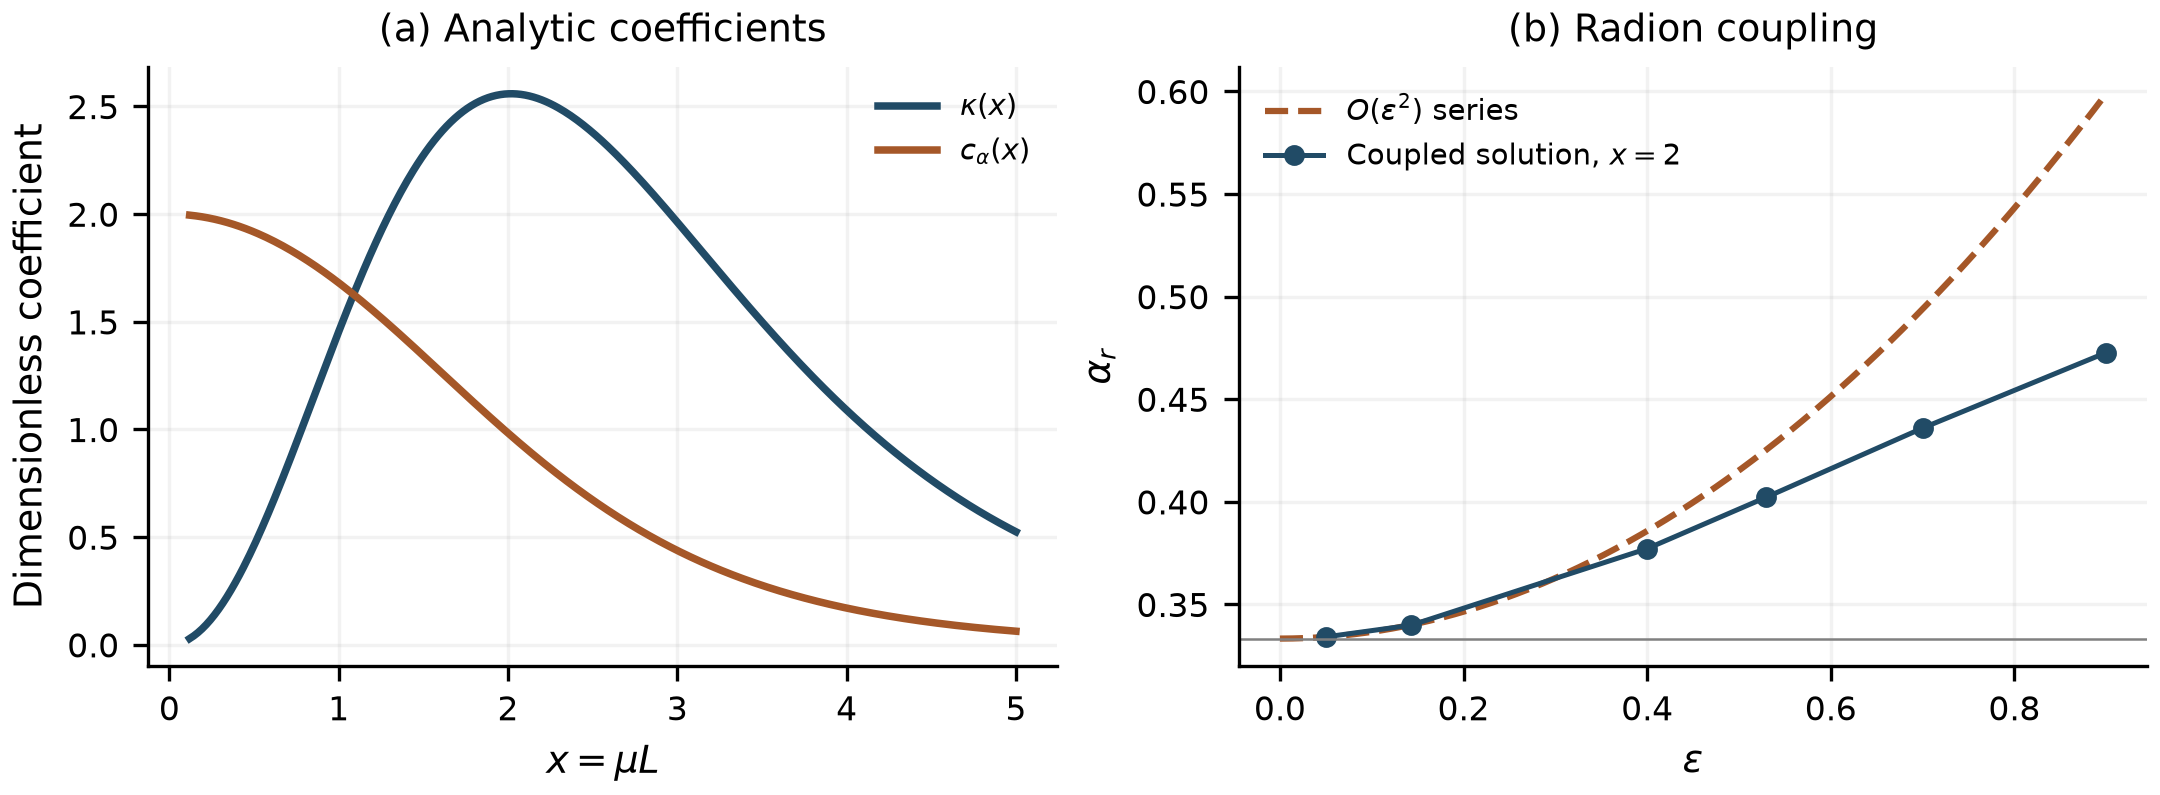
\includegraphics[width=\linewidth]{figures/weak_coupling.png}
\caption{Closed analytic coefficients and the finite-backreaction radion coupling at $x=2$. The truncated small-$\epsilon$ series is not exact at finite backreaction.}
\end{figure}
\section*{9. Exchange signal and its relation to short-distance gravity}
For normalized tensor profiles define I = \(\int\)e\({}^2\)\({}^A\)dy. The same-brane coupling of a massive tensor mode includes its massive spin-two polarization factor [10]:

\begin{equation}
\alpha_{T,n}=\frac43\frac{I\,h_n(0)^2}{\int_0^Le^{2A}h_n^2dy}.\tag{32}
\end{equation}
In the appropriate flat interval limit this yields \(\alpha\)T,n = 8/3 and mT,n = n\(\pi\)/L for n > 0. Backreaction changes both the profiles and the masses. Consequently, R\({}_0\) = L/\(\pi\) and the range 1/mT,1 need not coincide, as Table 2 illustrates.

For pointlike nonrelativistic sources on the same boundary, the correction to the potential relative to the massless tensor exchange is

\begin{equation}
V(r)=-\frac{G_Tm_1m_2}{r}\left[1+\Delta_V(r)\right],\tag{33}
\end{equation}
\begin{equation}
\Delta_V(r)=\sum_n\alpha_{s,n}e^{-m_{s,n}r}+\sum_{n>0}\alpha_{T,n}e^{-m_{T,n}r}.\tag{34}
\end{equation}
The relative correction to the attractive force magnitude contains an additional radial derivative:

\begin{equation}
\Delta_F(r)=\sum_n\alpha_{s,n}(1+m_{s,n}r)e^{-m_{s,n}r}+\sum_{n>0}\alpha_{T,n}(1+m_{T,n}r)e^{-m_{T,n}r}.\tag{35}
\end{equation}
These expressions are linear, static exchange formulas. A laboratory observable requires integration over the actual source and test-mass geometry and application of the experimental response and fit. The published single-Yukawa confidence curve in a torsion-balance analysis [11] is not a pointwise bound on \(\Delta\)V at r = \(\lambda\). A multimode signal must be evaluated in the appropriate experimental analysis. No exclusion contour or claim of agreement is supplied here.

The normalization GT refers to the massless tensor mode. If a scalar remains active at the distance used to infer Newton's constant, the conversion between GT and that measured constant must be included. If all additional exchanges have micrometric range while Newton's constant is determined macroscopically, their contribution at that reference distance is exponentially suppressed. This convention issue is separate from the actual data analysis.

\section*{10. Relation to earlier work and effective-theory limitations}
Neither reflection symmetry nor canonical radion coupling is itself new. Equal endpoint warp factors with a nontrivial interior have been considered previously [7], and exactly reflection-symmetric warped models with an odd stabilizing scalar and a radion spectrum are explicit in [8]. The distinction studied here is the chosen convex quadratic bulk potential, linear physical endpoint sources, reconstructed flat-slice branch, and the resulting closed coefficients and benchmarks. General normalization and fluctuation methods remain those of the established scalar--gravity literature [3,4,6].

A recent discussion of two linear brane potentials in an effective Randall--Sundrum description finds no nonzero-radius minimum in its approximation [9]. That comparison must retain its assumptions: its stated expansion is about an AdS/RS background with a negative bulk constant and a truncated weak-backreaction effective potential. The present branch instead has \(\Lambda\)\({}_5\) > 0 and a nonmonotonic warp factor. Equations (29)--(30) and the exact positive form (14) concern that different domain. They do not constitute a refutation of the RS calculation, nor do they support stabilization for arbitrary linear-brane models.

The calculation is classical and uses a two-derivative five-dimensional action. A physical application requires bulk curvature invariants and scalar-gradient energy to lie below the ultraviolet cutoff, control of boundary interactions and their radiative corrections, and a specification of the source-matter sector. Linear brane potentials are an imposed truncation, not a demonstrated radiatively protected structure. The negative endpoint background energies noted in Section 2 and the tuning needed for flat slices require a microscopic interpretation before a complete compactification claim can be made.

Small spacetime curvature is not by itself control of an arbitrary scalar potential. At x = 2, the endpoint field amplitudes \(\sigma\)b/M\({}_5\)\({}^3\)\({}^{/}\)\({}^2\) are approximately 0.489, 0.621 and 0.924 at \(\epsilon\) = 0.4, 0.53 and 0.9. The last value is close to the gravitational field scale in this convention. A quadratic potential therefore needs a protective mechanism or an explicit bound on higher scalar operators before the strongest-backreaction benchmarks can be treated as a robust microscopic prediction. The numerical results remain well-defined outputs of the specified truncated classical action.

The current model also does not calculate the absolute length. Micrometric extra dimensions have independent theoretical motivations in the literature [12], but those motivations do not fix the stabilizer parameters of (1). A proposed connection to DDF geometry must supply the effective action, its dimensional coefficients and boundary data before the spectrum here becomes a prediction of that geometry. The recovery of a consistent effective sector should be assessed separately from broader historical DDF claims.

\section*{11. Conclusions}
A reflection-symmetric physical interval with a canonical scalar, a convex quadratic bulk potential and linear endpoint potentials admits a regular scalar spectral formulation through the interior zero of the warp derivative. For every smooth branch point with \(\mu\) > 0 and q > 0, the endpoint signs make the generalized norm positive and establish strictly positive scalar squared masses. The canonical scalar norm is independently positive; the transverse tensor sector has one massless mode and positive massive excitations.

At fixed x = \(\mu\)L, the light radion has m\({}_r\)\({}^2\)L\({}^2\) = \(\kappa\)(x)\(\epsilon\)\({}^2\) + O(\(\epsilon\)\({}^4\)), with \(\kappa\) = 4x tanh(x/2)sech\({}^2\)(x/2). Its minimally coupled same-brane Yukawa amplitude is \(\alpha\)\({}_r\) = [1 + c\(\alpha\)(x)\(\epsilon\)\({}^2\) + O(\(\epsilon\)\({}^4\))]/3, with c\(\alpha\) = sech\({}^2\)(x/2)[1 + tanh\({}^2\)(x/2) + 2tanh(x/2)/x] > 0. A separate weak-backreaction effective-potential calculation reproduces the mass coefficient. Finite-backreaction benchmarks illustrate why masses and normalized residues must be computed together.

These results characterize the stated effective family and its perturbations. They leave the absolute compactification length, ultraviolet completion, full experimental response, and derivation from DDF geometry unresolved. The reproducible coefficients and stability check provide a concrete basis for a focused theoretical article without converting those open questions into established predictions.

\section*{Appendix A. Elementary integrals and normalization check}
The three integrals entering (25) can be evaluated directly from (24). With C = cosh\({}^2\)(x/2), T = tanh(x/2), and averaging over -1/2 \(\leq\) t \(\leq\) 1/2, they are

\begin{equation}
f_2(1/2)=\frac{1+2T/x}{C},\tag{A1}
\end{equation}
\begin{equation}
\langle f_2\rangle=\frac{1/3+1/x^2-\sinh(x)/x^3+T/x}{C},\tag{A2}
\end{equation}
\begin{equation}
\langle s_1^2\rangle=\frac{12}{C}\left[\frac16-\frac{T^2}{2}-\frac1{x^2}+\frac{\sinh x}{x^3}\right].\tag{A3}
\end{equation}
Substitution into (25) cancels the inverse-square and hyperbolic-cubic terms and gives (26). The accompanying standard-library script independently integrates the unsimplified profiles with composite Simpson quadrature at x = 0.5, 1, 2, 3 and 4, checks the endpoint condition xTb(1/2) = \(\kappa\), and compares the averages with (A1)--(A3). This quadrature is independent of the finite-backreaction spectral solver.

For the canonical-norm identity, insert s = -3M\({}_5\)\({}^3\)e\({}^-\)\({}^2\)\({}^A\)g\({}^\prime\)/\(\sigma\)\({}^\prime\) and f = e\({}^-\)\({}^2\)\({}^A\)g in (18). The result is

\begin{equation}
N_f=\frac{9M_5^6}{2}\int_0^L\left[p(g^\prime)^2+Qg^2\right]dy=\frac{9M_5^6}{2}m^2\mathcal{D}[g].\tag{A4}
\end{equation}
The identity checks dimensions and normalization, but the source amplitude remains (20). In particular, replacing Nf by \(\mathcal D\)[g] alone loses a mass-dependent factor. Direct matter couplings, additional kinetic boundary terms, or a different physical-interval counting would require rederivation.

\section*{Research and data statement}
This is a first research draft dated 5 September 2026, not a peer-reviewed publication. The accompanying repository contains the active model conventions, analytical derivations, machine-readable benchmark results, numerical reproduction scripts, and a separated historical archive. Historical documents are provenance, not additional premises of this article. Numerical precision and model-dependent conclusions are explicitly distinguished from physical validation.

AI tools assisted drafting, algebraic checks, numerical implementation and literature screening. Scientific responsibility remains with the named author, who must review and approve the scientific content before submission. Bibliographic priority, the physical interpretation of the boundary sources, and independent expert review remain to be assessed. No affiliation or funding claim is made in this draft.

\begin{thebibliography}{99}
\bibitem{GW1999} W. D. Goldberger and M. B. Wise, Modulus Stabilization with Bulk Fields, Physical Review Letters 83, 4922--4925 (1999). DOI: 10.1103/PhysRevLett.83.4922. arXiv: hep-ph/9907447.
\bibitem{DFGK2000} O. DeWolfe, D. Z. Freedman, S. S. Gubser and A. Karch, Modeling the fifth dimension with scalars and gravity, Physical Review D 62, 046008 (2000). DOI: 10.1103/PhysRevD.62.046008. arXiv: hep-th/9909134.
\bibitem{CGK2001} C. Csáki, M. L. Graesser and G. D. Kribs, Radion Dynamics and Electroweak Physics, Physical Review D 63, 065002 (2001). DOI: 10.1103/PhysRevD.63.065002. arXiv: hep-th/0008151.
\bibitem{KMP2004} L. Kofman, J. Martin and M. Peloso, Exact identification of the radion and its coupling to the observable sector, Physical Review D 70, 085015 (2004). DOI: 10.1103/PhysRevD.70.085015. arXiv: hep-ph/0401189.
\bibitem{LS2004} J. Lesgourgues and L. Sorbo, Goldberger-Wise variations: stabilizing brane models with a bulk scalar, Physical Review D 69, 084010 (2004). DOI: 10.1103/PhysRevD.69.084010. arXiv: hep-th/0310007.
\bibitem{O2025} M. Olechowski, Stability of multibrane models, Nuclear Physics B 1011, 116807 (2025). DOI: 10.1016/j.nuclphysb.2025.116807. arXiv: 2408.15343.
\bibitem{Boos2005} E. E. Boos, Y. S. Mikhailov, M. N. Smolyakov and I. P. Volobuev, Energy scales in a stabilized brane world, Nuclear Physics B 717, 19--33 (2005). DOI: 10.1016/j.nuclphysb.2005.04.012. arXiv: hep-th/0412204.
\bibitem{MP2011} A. D. Medina and E. Pontón, Warped Universal Extra Dimensions, Journal of High Energy Physics 06 (2011), 009. DOI: 10.1007/JHEP06(2011)009. arXiv: 1012.5298.
\bibitem{LNR2026} S. Lüst, M. Nee and L. Randall, More effective RS field theory, Journal of High Energy Physics 06 (2026), 130. DOI: 10.1007/JHEP06(2026)130. arXiv: 2510.11771; comparison uses preprint v2.
\bibitem{CR2004} P. Callin and F. Ravndal, Higher order corrections to the Newtonian potential in the Randall-Sundrum model, Physical Review D 70, 104009 (2004). DOI: 10.1103/PhysRevD.70.104009. arXiv: hep-ph/0403302.
\bibitem{Lee2020} J. G. Lee, E. G. Adelberger, T. S. Cook, S. M. Fleischer and B. R. Heckel, New Test of the Gravitational 1/r\({}^2\) Law at Separations down to 52 \(\mu\)m, Physical Review Letters 124, 101101 (2020). DOI: 10.1103/PhysRevLett.124.101101. arXiv: 2002.11761.
\bibitem{MVV2023} M. Montero, C. Vafa and I. Valenzuela, The Dark Dimension and the Swampland, Journal of High Energy Physics 02 (2023), 022. DOI: 10.1007/JHEP02(2023)022. arXiv: 2205.12293.
\end{thebibliography}
\end{document}
